\providecommand{\setflag}{\newif \ifwhole \wholefalse}
\setflag
\ifwhole\else

% Typography and geometry ----------------------------------------------------
\documentclass[letterpaper]{scrbook}
\usepackage[inner=3cm,top=2.5cm,outer=3.5cm]{geometry}

\renewcommand\familydefault{bch}
\usepackage[utf8]{inputenc}
\usepackage{microtype}
\usepackage[small]{caption}
\usepackage[small]{titlesec}
\raggedbottom

% Graphics -------------------------------------------------------------------
\usepackage[pdftex]{graphicx}
\graphicspath{{_include/}}
\DeclareGraphicsExtensions{.png,.pdf}

% Code formatting ------------------------------------------------------------
\usepackage{fancyvrb}
\usepackage{courier}
\usepackage{listings}
\usepackage{color}
\usepackage{alltt}


\definecolor{comment}{rgb}{0.60, 0.60, 0.53}
\definecolor{background}{rgb}{0.97, 0.97, 1.00}
\definecolor{string}{rgb}{0.863, 0.066, 0.266}
\definecolor{number}{rgb}{0.0, 0.6, 0.6}
\definecolor{variable}{rgb}{0.00, 0.52, 0.70}
\lstset{
  basicstyle=\ttfamily,
  keywordstyle=\bfseries, 
  identifierstyle=,  
  commentstyle=\color{comment} \emph,
  stringstyle=\color{string},
  showstringspaces=false,
  columns = fullflexible,
  backgroundcolor=\color{background},
  mathescape = true,
  escapeinside=&&,
  fancyvrb
}
\newcommand{\code}[1]{\lstinline!#1!}
\newcommand{\f}[1]{\lstinline!#1()!}



% Links ----------------------------------------------------------------------

\usepackage{hyperref}
\definecolor{slateblue}{rgb}{0.07,0.07,0.488}
\hypersetup{colorlinks=true,linkcolor=slateblue,anchorcolor=slateblue,citecolor=slateblue,filecolor=slateblue,urlcolor=slateblue,bookmarksnumbered=true,pdfview=FitB}
\usepackage{url}

% Tables ---------------------------------------------------------------------
\usepackage{longtable}
\usepackage{booktabs}

% Miscellaneous --------------------------------------------------------------
\usepackage{pdfsync}
\usepackage{appendix}

\usepackage[round,sort&compress,sectionbib]{natbib}
\bibliographystyle{plainnat}


\title{ggplot2}
\author{Hadley Wickham}

\begin{document}
\fi


% SET_DEFAULTS
%   GG-WIDTH: 4  GG-HEIGHT: 4
%   TEX-WIDTH: 0.5\linewidth
%   INLINE: FALSE
% 

% END

\chapter{Manipulating plot rendering with \code{grid}}
\label{cha:grid}

\section{Introduction}

Sometimes you may need to go beyond the theming system and directly modify the underlying grid graphics output.  To do this, you will need a good understanding of grid, as described in ``R Graphics'' \citep{murrell:2005}.  If you can't get the book, at least read Chapter 5, ``The grid graphics model'', which is available online for free at  \url{http://www.stat.auckland.ac.nz/~paul/RGraphics/chapter5.pdf}.  This appendix outlines the more important viewports and grobs used by \ggplot and should be helpful if you need to modify the plot.

\section{Plot viewports}
\label{sec:plot-viewports}

Viewports define the basic regions of the plot.  The structure will vary slightly from plot to plot, depending on the type of faceting used, but the basics will remain the same. 

The {\tt panels} viewport contains the meat of the plot: strip labels, axes and faceted panels.  The viewports are named according to both their job and their position on the plot.  A prefix (listed below) describes the contents of the viewport, and is followed by integer x and y position (counting from bottom left) separated by ``\_''.  Figure~\ref{fig:panelvp} illustrates this naming scheme for a 2$\times$2 plot.

\begin{itemize}
  \item {\tt strip\_h}: horizontal strip labels
  \item {\tt strip\_v}: vertical strip labels
  \item {\tt axis\_h}: horizontal axes
  \item {\tt axis\_v}: vertical axes
  \item {\tt panel}: faceting panels
\end{itemize}

\begin{figure}[htbp]
  \centering
    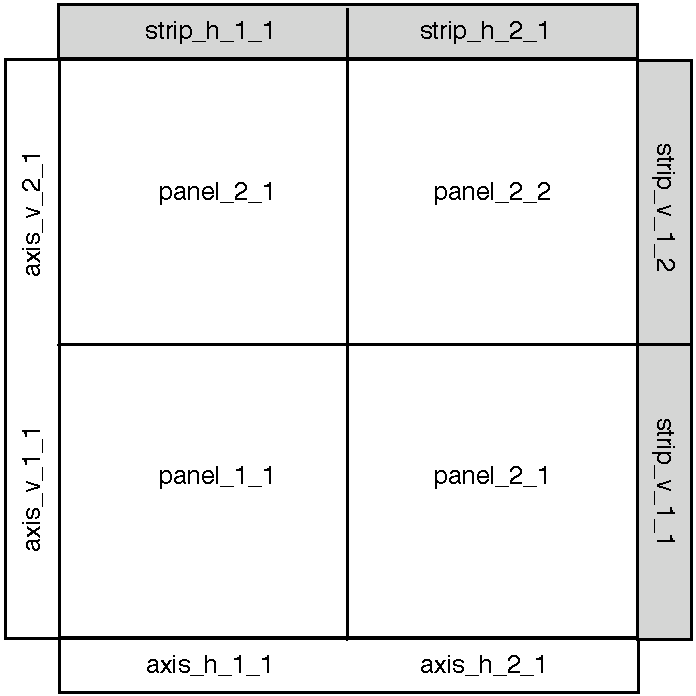
\includegraphics[width=0.5 \linewidth]{grid-panelvp}
  \caption{Naming scheming of the panel viewports}
  \label{fig:panelvp}
\end{figure}

The \code{panels} viewport is contained inside the \code{background} viewport which also contains the following viewports:

\begin{itemize}
  \item \code{title}, \code{xlabel}, and \code{ylabel}: for the plot title, and x and y axis labels
  \item \code{legend_box}: for all of the legends for the plot
\end{itemize}

\noindent Figure~\ref{fig:viewports} labels a plot with a representative sample of these viewports.  To get a list of all viewports on the current plot, run \code{current.vpTree(all=TRUE)} or \code{grid.ls(grobs = FALSE, viewports = TRUE)}.

\begin{figure}[htbp]
  \centering
    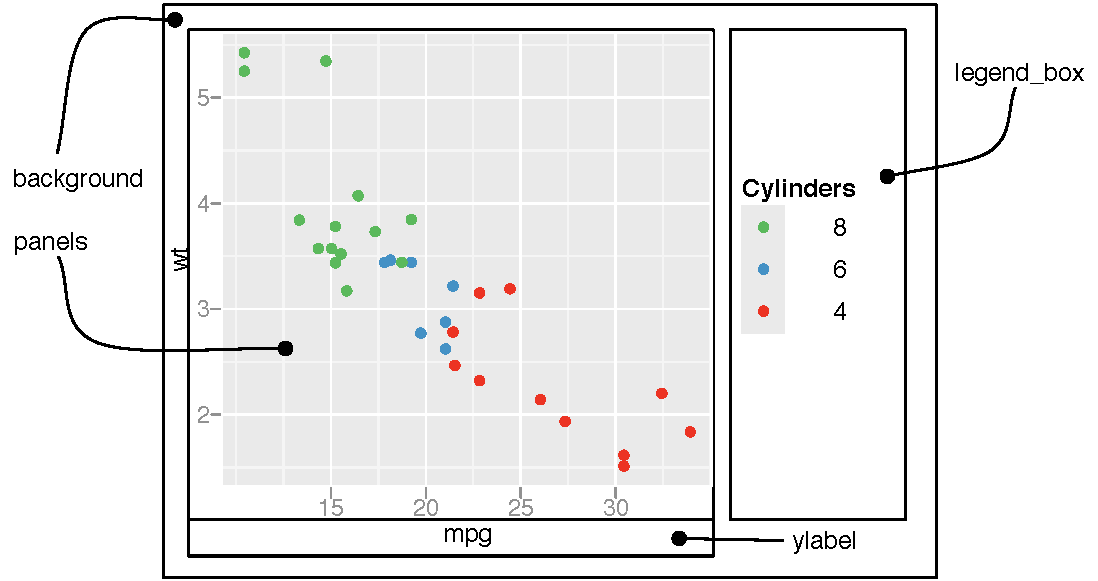
\includegraphics[width=\linewidth]{grid-viewports}
  \caption{Diagram showing the structure and names of viewports.}
  \label{fig:viewports}
\end{figure}

\section{Plot grobs}
\label{sec:plot-grobs}

Grob names have three components: the name of the grob, the class of the grob, and a unique numeric suffix.  The three components are joined together with ``.'' to give a name like {\tt title.text.435} or {\tt ticks.segments.15}.  These three components ensure that all grob names are unique, and allow you to select multiple grobs with the same name at the same time.  Figure~\ref{fig:grobs} labels some of these grobs.  The grobs are arranged hierarchically, but it's hard to capture this in a diagram.  You can see a list of all the grobs in the current plot with {\tt grid.ls()}.  

\begin{figure}[htbp]
  \centering
    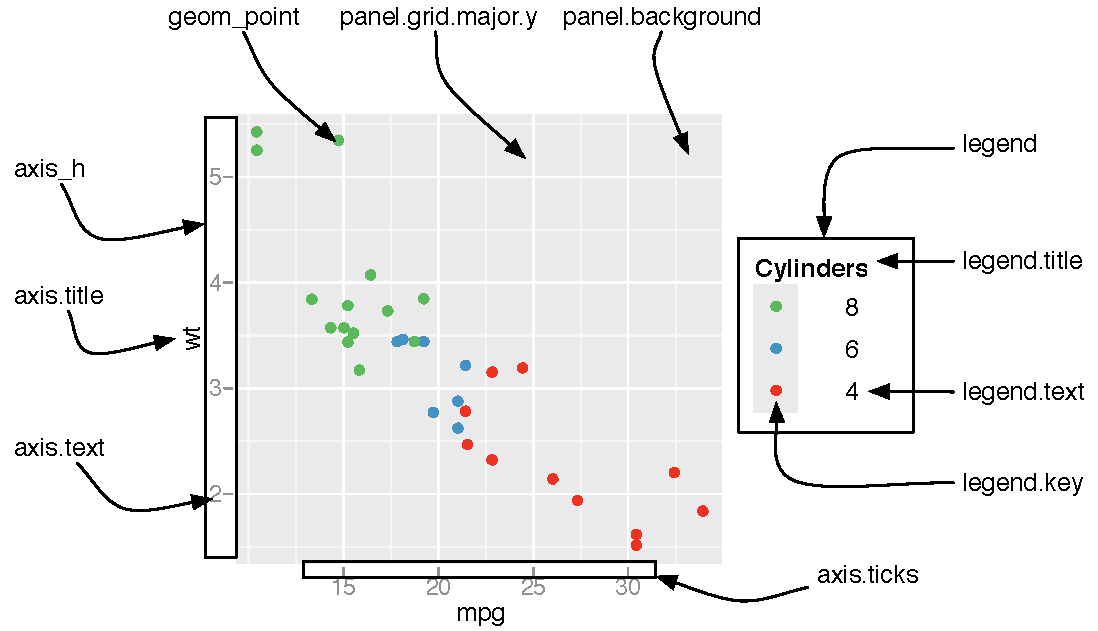
\includegraphics[width=\linewidth]{grid-grobs}
  \caption{A selection of the most important grobs.}
  \label{fig:grobs}
\end{figure}


% \section{Editing existing objects on the plot}
% \label{sec:grid-existing}
% 
% From time to time, the theming system will not give you enough control.  This may occur if you want to modify a single element of a plot, like one grid line or a single label.  Where possible, using the theming system will be easier, because using grid will affect a component, but not the space saved for that element.
% 
% Most of the difficulty in modifying elements of the plot is figuring out what the grob you want to modify is called.  Once you have that you can use {\tt grid.gedit}, to locate and then modify that grob. 
% 
% To fully identify a grob, you need to use a \code{gPath}.  A \code{gPath} can either be a string specifying a single grob name, or a sequence of grob names that describe hierarchy to travel down to get to the grob of interest with the {\tt gPath} function.  Using a string will find all grobs with that name regardless of their position in the hierarchy.  For example, {\tt "label"} will find all grobs called label, regardless of where they are.  To be more specific, using {\tt gPath("parent", "child")} will only find grobs named ``child'' with a parent called ``parent''.  For example, {\tt gPath("xaxis", "label")} will locate only labels on the x-axis.
% 
% Modifying a grob requires some knowledge of the different parameters of the grob.  This is where the second part of the grob name is useful, as it will tell you whether you are modifying a line, or a rect or a text grob.  You can get more information by looking at the documentation for that grob, eg. {\tt ?grid.rect, ?grid.text, ?grid.lines}   As well as individual parameters, all grobs share a common set of graphical parameters described in Table \ref{tbl:gpar}. Appendix~\ref{cha:specifications} describes the values that these may take.
% 
% \begin{table}
%   \begin{center}
%   \begin{tabular}{lll}
%     \toprule
%     Grid parameter & \ggplot aesthetic &  Description \\
%     \midrule
%     lwd & size & Line width (in pts) \\
%     col & colour & Border colour \\
%     fill  & fill & Fill colour \\
%     fontsize & size & Font size (in pts) \\
%     fontface & --- & Font face (bold, italic, ...) \\
%     \bottomrule
%   \end{tabular}
%   \end{center}
%   \caption{Common graphical parameters for grid grobs.  Note that point size is controlled separately.}
%   \label{tbl:gpar}
% \end{table}
% 
% In this example, we edit the font of all labels.
% 
% \begin{alltt}
% qplot(mpg, wt, data = mtcars, facets = . ~ cyl)
% 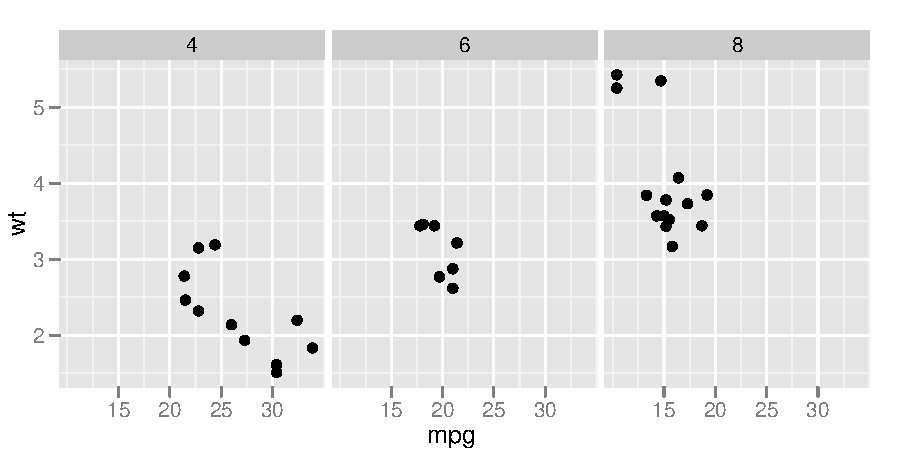
\includegraphics[width=0.75\linewidth]{grid1}
% grid.gedit("text", gp = gpar(fontsize=14, col="red"))
% 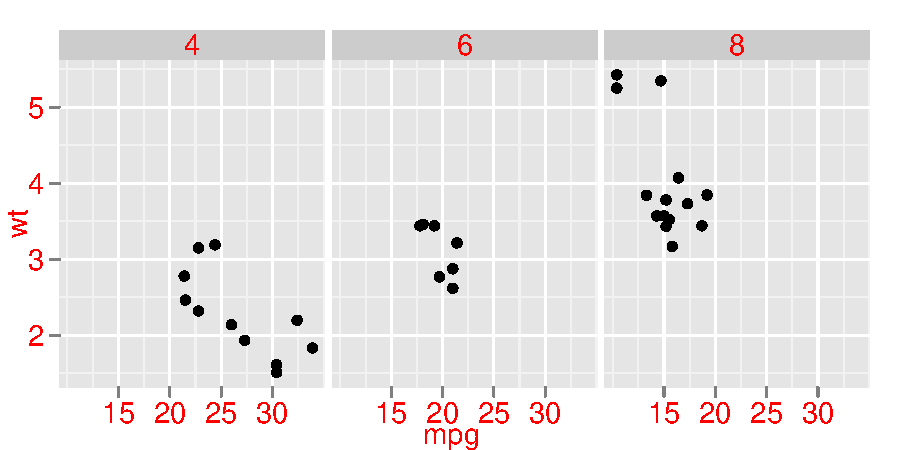
\includegraphics[width=0.75\linewidth]{grid2}
% \end{alltt}
% % dev.copy2pdf(file = "grid1.pdf", width = 6, height = 3)
% % dev.copy2pdf(file = "grid2.pdf", width = 6, height = 3)
% 
% To edit just one type of label, we need to use the hierarchy of grobs and the {\tt gPath} function:
% 
% \begin{alltt}
% qplot(mpg, wt, data = mtcars, facets = . ~ cyl)
% grid.gedit(gPath("strip","text"), gp = gpar(fontface="bold"))
% 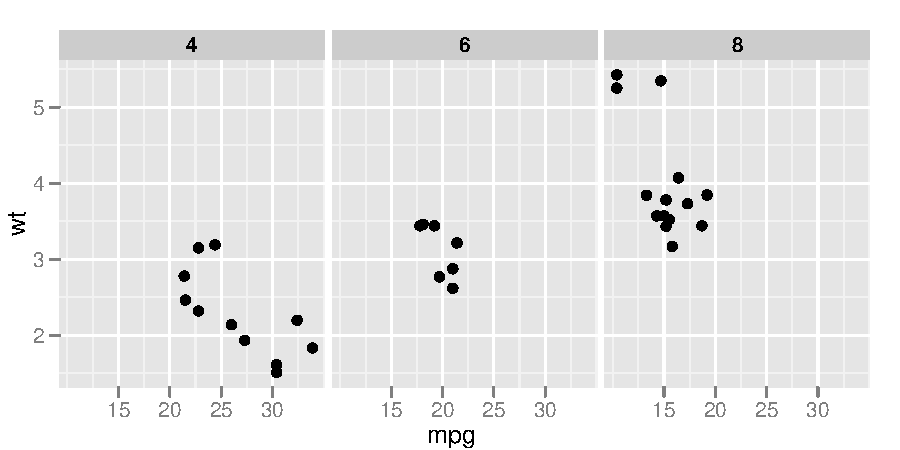
\includegraphics[width=0.75\linewidth]{grid3}
% grid.gedit(gPath("axis_h", "text"), gp = gpar(col="red"))
% 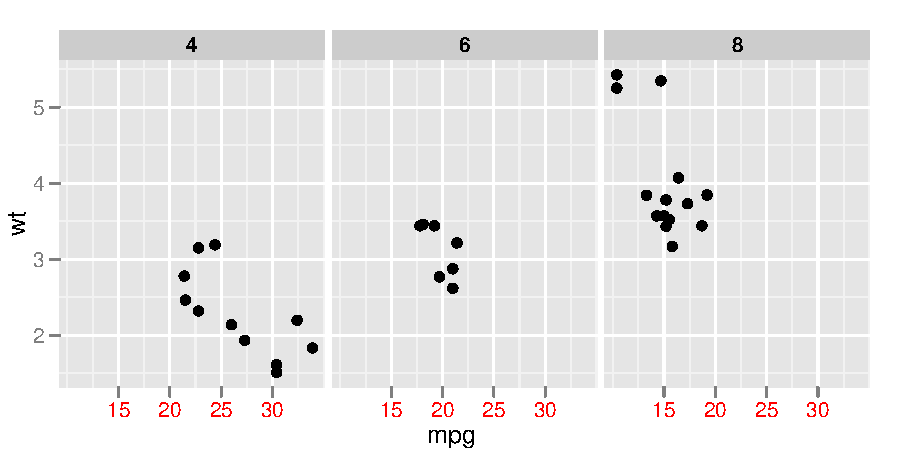
\includegraphics[width=0.75\linewidth]{grid4}
% \end{alltt}
% % dev.copy2pdf(file = "grid3.pdf", width = 6, height = 3)
% % dev.copy2pdf(file = "grid4.pdf", width = 6, height = 3)


\section{Saving your work} 
\label{sec:grid-save}

Using \f{grid.gedit} works fine if you are editing the plot on screen, but if you want to save it to disk you need take some extra steps, or you will end up with multiple pages of output, each showing one change.  The key is not to modify the plot on screen, but to modify the plot grob, and then draw it once you have made all the changes.  

% LISTING
% 
% p <- qplot(wt, mpg, data=mtcars, colour=cyl)
% # Get the plot grob
% grob <- ggplotGrob(p)
% # Modify in place
% grob <- geditGrob(grob, gPath("strip","label"), gp=gpar(fontface="bold"))
% 
% # Draw it
% grid.newpage()
% grid.draw(grob)
\input{_include/65cedb19a8e6185946376cdd40cc7311.tex}
% END

An alternative is make all of the changes on screen, and then use \f{dev.copy2pdf} to copy the final version to disk.

\ifwhole
\else
  \nobibliography{/Users/hadley/documents/phd/references}
  \end{document}
\fi
